\documentclass[tikz]{standalone}

\usetikzlibrary{decorations.pathreplacing}

\definecolor{axis color}{RGB}{200,10,0}
\definecolor{accum color}{RGB}{0,150,10}
\definecolor{flow color}{RGB}{10,30,245}
\definecolor{flow fill}{RGB}{200, 215, 255}

\begin{document}
	
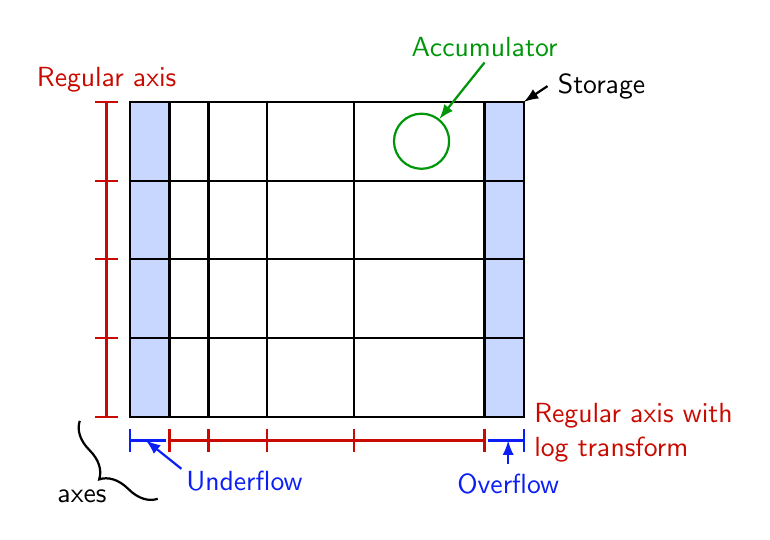
\begin{tikzpicture}[
	font=\sffamily,
	thick]

% Shading
\path [fill=flow fill] (-2.5, -2) rectangle (-2, 2);
\path [fill=flow fill] (2.5, -2) rectangle (2, 2);

% Main grid
\draw (-2.5,-2) rectangle (2.5,2);
\foreach \i in {-1,0,1} {
    \draw (-2.5,\i) -- (2.5,\i);
}
\foreach \i in {-2, -1.50465122, -0.76393202,  0.34370152, 2} {
    \draw (\i, -2) -- (\i, 2);
}

\draw [latex-] (2.5,2) -- (2.8,2.2) node [right] {Storage};

% Left axis
\draw [axis color] (-2.8,-2) -- (-2.8,2);
\foreach \i in {-2,-1,0,1,2} {
    \draw [axis color] (-2.95,\i) -- (-2.65,\i);
}
\node at (-2.8,2) [above, axis color] {Regular axis};

% Bottom axis
\draw [axis color] (-2,-2.3) -- (2,-2.3);
\foreach \i in {-2.        , -1.50465122, -0.76393202,  0.34370152,  2.} {
    \draw [axis color] (\i, -2.45) -- (\i, -2.15);
}
\node at (2,-2.2) [axis color, right=.5cm, align=left] {Regular axis with\\log transform};

% Axes
\begin{scope}[xshift=-2.9cm, yshift=-2.8cm, rotate=45]
\draw [decorate, decoration={brace,amplitude=10pt}, xshift=-4pt, yshift=0pt]
    (0.5,-0.7) -- (0.5,0.7);
\node at (-.3,0) {axes};
\end{scope}

% Overflow bin
\draw [flow color] (2.05,-2.3) -- (2.5, -2.3);
\draw [flow color] (2.5, -2.45) -- (2.5, -2.15);
\draw [flow color, latex- ] (2.3, -2.3) -- (2.3, -2.6) node [below] {Overflow};

% Underflow bin
\draw [flow color] (-2.05,-2.3) -- (-2.5, -2.3);
\draw [flow color] (-2.5, -2.45) -- (-2.5, -2.15);
\draw [flow color, latex- ] (-2.3, -2.3) -- (-1.85, -2.66) node [below=-.1cm, xshift=.8cm] {Underflow};

% Accumulators
\node (accum) at (1.2,1.5) [circle, minimum width=.7cm, draw, accum color] {};
\draw [accum color, latex-] (accum) -- (2, 2.5) node [above=-.05cm] {Accumulator};

\end{tikzpicture}

\end{document}